\documentclass[tikz,border=12pt]{standalone}
\usepackage[utf8]{inputenc}
\usepackage[T1]{fontenc}
\usepackage{lmodern}
\usepackage{amsmath}
\usetikzlibrary{arrows.meta,positioning,fit,backgrounds,shapes.geometric}

\definecolor{coseblue}{RGB}{0,70,140}
\definecolor{coseteal}{RGB}{22,138,128}
\definecolor{coseamber}{RGB}{217,119,6}
\definecolor{cosered}{RGB}{185,28,28}
\definecolor{slatebg}{RGB}{248,250,252}
\definecolor{slateborder}{RGB}{148,163,184}
\definecolor{lecadark}{RGB}{71,85,105}
\definecolor{lecashell}{RGB}{203,213,225}

\begin{document}
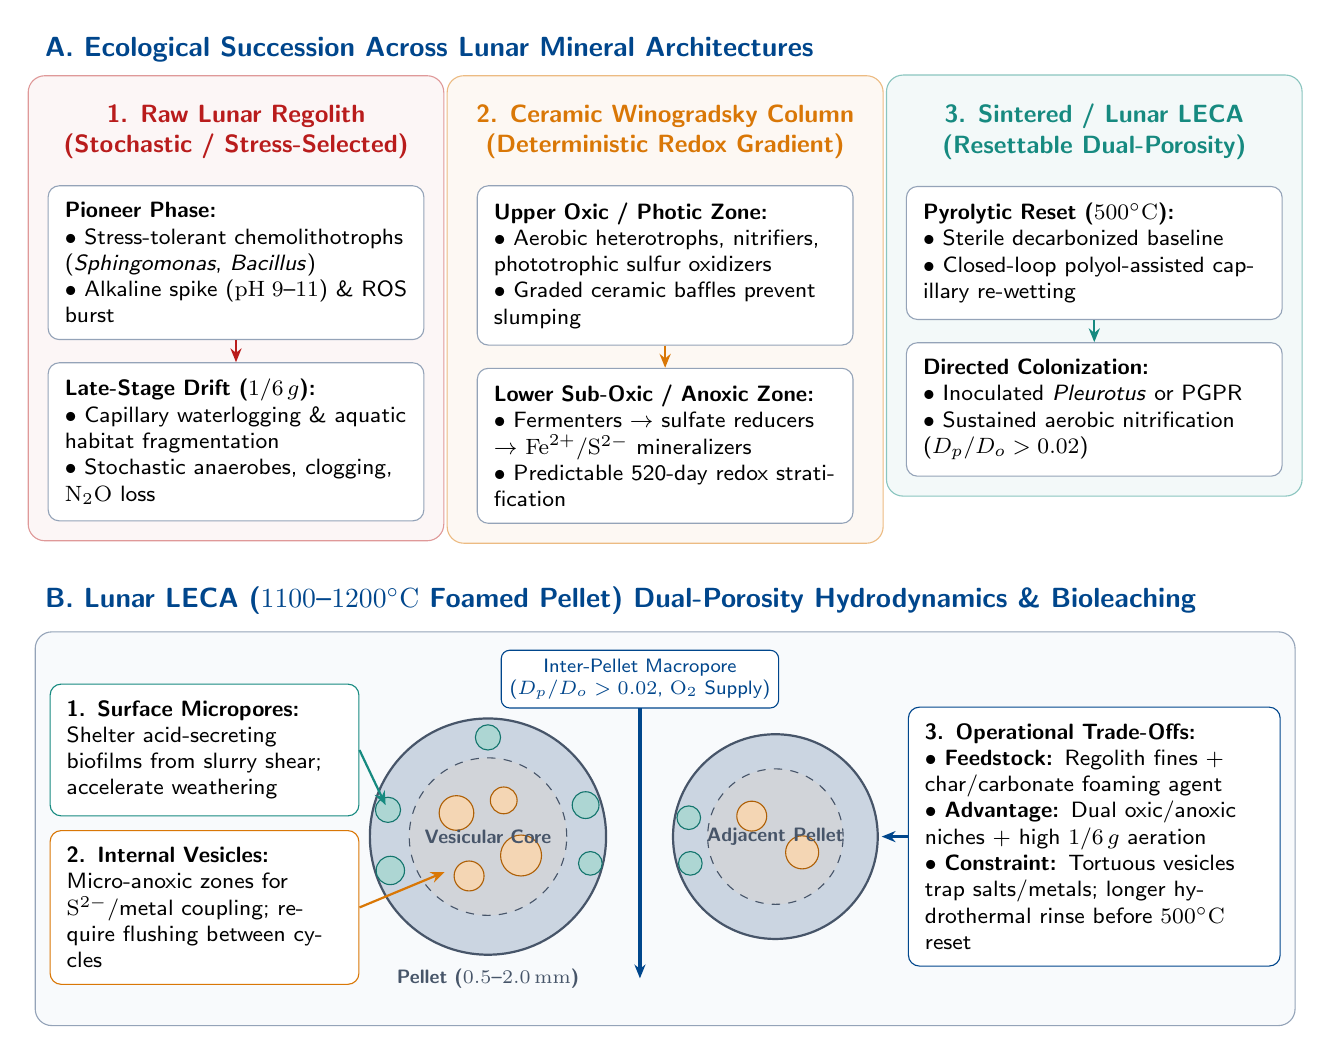
\begin{tikzpicture}[
    font=\sffamily\small,
    paneltitle/.style={
        font=\sffamily\bfseries\normalsize,
        text=coseblue,
        anchor=west
    },
    coltitle/.style={
        font=\sffamily\bfseries\small,
        align=center
    },
    subbox/.style={
        draw=slateborder,
        rounded corners=4pt,
        fill=white,
        inner sep=6pt,
        align=left,
        font=\sffamily\footnotesize,
        text width=4.35cm
    },
    arrow/.style={
        -{Stealth[length=5pt,width=4pt]},
        thick
    }
]

% =========================================================================
% PANEL A: MICROBIAL SUCCESSION TRAJECTORIES
% =========================================================================
\node[paneltitle] (pa) at (-8.0, 5.95) {A. Ecological Succession Across Lunar Mineral Architectures};

% Column 1: Raw Regolith
\node[coltitle, text=cosered] (c1t) at (-5.45, 4.9) {1. Raw Lunar Regolith\\(Stochastic / Stress-Selected)};
\node[subbox, below=6pt of c1t] (c1a) {
    \textbf{Pioneer Phase:}\\
    $\bullet$ Stress-tolerant chemolithotrophs (\textit{Sphingomonas}, \textit{Bacillus})\\
    $\bullet$ Alkaline spike ($\mathrm{pH}\;9\text{--}11$) \& ROS burst
};
\node[subbox, below=8pt of c1a] (c1b) {
    \textbf{Late-Stage Drift ($1/6\,g$):}\\
    $\bullet$ Capillary waterlogging \& aquatic habitat fragmentation\\
    $\bullet$ Stochastic anaerobes, clogging, $\mathrm{N}_2\mathrm{O}$ loss
};
\draw[arrow, draw=cosered] (c1a.south) -- (c1b.north);

% Column 2: Winogradsky Column
\node[coltitle, text=coseamber] (c2t) at (0.0, 4.9) {2. Ceramic Winogradsky Column\\(Deterministic Redox Gradient)};
\node[subbox, below=6pt of c2t] (c2a) {
    \textbf{Upper Oxic / Photic Zone:}\\
    $\bullet$ Aerobic heterotrophs, nitrifiers, phototrophic sulfur oxidizers\\
    $\bullet$ Graded ceramic baffles prevent slumping
};
\node[subbox, below=8pt of c2a] (c2b) {
    \textbf{Lower Sub-Oxic / Anoxic Zone:}\\
    $\bullet$ Fermenters $\rightarrow$ sulfate reducers $\rightarrow$ $\mathrm{Fe}^{2+}/\mathrm{S}^{2-}$ mineralizers\\
    $\bullet$ Predictable 520-day redox stratification
};
\draw[arrow, draw=coseamber] (c2a.south) -- (c2b.north);

% Column 3: Porous Ceramic / Lunar LECA
\node[coltitle, text=coseteal] (c3t) at (5.45, 4.9) {3. Sintered / Lunar LECA\\(Resettable Dual-Porosity)};
\node[subbox, below=6pt of c3t] (c3a) {
    \textbf{Pyrolytic Reset ($500^\circ\mathrm{C}$):}\\
    $\bullet$ Sterile decarbonized baseline\\
    $\bullet$ Closed-loop polyol-assisted capillary re-wetting
};
\node[subbox, below=8pt of c3a] (c3b) {
    \textbf{Directed Colonization:}\\
    $\bullet$ Inoculated \textit{Pleurotus} or PGPR\\
    $\bullet$ Sustained aerobic nitrification ($D_p/D_o > 0.02$)
};
\draw[arrow, draw=coseteal] (c3a.south) -- (c3b.north);

\begin{scope}[on background layer]
    \node[draw=cosered!45, fill=cosered!4, rounded corners=6pt, inner sep=7pt, fit=(c1t)(c1a)(c1b)] {};
    \node[draw=coseamber!50, fill=coseamber!5, rounded corners=6pt, inner sep=7pt, fit=(c2t)(c2a)(c2b)] {};
    \node[draw=coseteal!50, fill=coseteal!5, rounded corners=6pt, inner sep=7pt, fit=(c3t)(c3a)(c3b)] {};
\end{scope}

% =========================================================================
% PANEL B: LUNAR LECA DUAL-POROSITY MECHANISM
% =========================================================================
\node[paneltitle] (pb) at (-8.0, -1.05) {B. Lunar LECA ($1100\text{--}1200^\circ\mathrm{C}$ Foamed Pellet) Dual-Porosity Hydrodynamics \& Bioleaching};

% Background box for Panel B
\node[draw=slateborder, fill=slatebg, rounded corners=6pt, minimum width=16.0cm, minimum height=5.0cm] (pbbox) at (0, -3.95) {};

% Pellet 1 (left-center cross section)
\begin{scope}[shift={(-2.25, -4.05)}]
    % Outer rough vesicular shell
    \fill[lecashell, draw=lecadark, thick] (0,0) circle (1.50cm);
    % Inner sintered core
    \fill[lecadark!25, draw=lecadark, dashed] (0,0) circle (1.00cm);
    % Closed internal vesicles (anoxic)
    \fill[coseamber!30, draw=coseamber!80!black] (-0.40, 0.30) circle (0.22cm);
    \fill[coseamber!30, draw=coseamber!80!black] (0.42, -0.24) circle (0.26cm);
    \fill[coseamber!30, draw=coseamber!80!black] (-0.24, -0.50) circle (0.19cm);
    \fill[coseamber!30, draw=coseamber!80!black] (0.20, 0.46) circle (0.17cm);
    % Open surface micropores (biofilm shelters)
    \fill[coseteal!35, draw=coseteal!85!black] (1.24, 0.40) circle (0.17cm);
    \fill[coseteal!35, draw=coseteal!85!black] (1.30, -0.34) circle (0.15cm);
    \fill[coseteal!35, draw=coseteal!85!black] (-1.27, 0.34) circle (0.16cm);
    \fill[coseteal!35, draw=coseteal!85!black] (-1.24, -0.43) circle (0.18cm);
    \fill[coseteal!35, draw=coseteal!85!black] (0.0, 1.26) circle (0.16cm);
    \node[font=\sffamily\bfseries\scriptsize, text=lecadark] at (0, 0) {Vesicular Core};
    \node[font=\sffamily\scriptsize, text=lecadark] at (0, -1.80) {\textbf{Pellet ($0.5\text{--}2.0\,\mathrm{mm}$)}};
\end{scope}

% Pellet 2 (adjacent pellet to show inter-aggregate macropore)
\begin{scope}[shift={(1.40, -4.05)}]
    \fill[lecashell, draw=lecadark, thick] (0,0) circle (1.30cm);
    \fill[lecadark!25, draw=lecadark, dashed] (0,0) circle (0.86cm);
    \fill[coseamber!30, draw=coseamber!80!black] (-0.30, 0.26) circle (0.19cm);
    \fill[coseamber!30, draw=coseamber!80!black] (0.34, -0.20) circle (0.21cm);
    \fill[coseteal!35, draw=coseteal!85!black] (-1.10, 0.24) circle (0.15cm);
    \fill[coseteal!35, draw=coseteal!85!black] (-1.08, -0.34) circle (0.15cm);
    \node[font=\sffamily\bfseries\scriptsize, text=lecadark] at (0, 0) {Adjacent Pellet};
\end{scope}

% Gas/Air flow arrow between pellets
\draw[arrow, draw=coseblue, line width=1.4pt] (-0.32, -2.35) -- (-0.32, -5.85);
\node[fill=white, draw=coseblue, rounded corners=3pt, inner sep=3pt, font=\sffamily\scriptsize, text=coseblue, align=center] at (-0.32, -2.05) {Inter-Pellet Macropore\\($D_p/D_o > 0.02$, $\mathrm{O}_2$ Supply)};

% Callouts on Left (Surface & Core)
\node[subbox, text width=3.5cm, draw=coseteal] (call1) at (-5.85, -2.95) {
    \textbf{1. Surface Micropores:}\\
    Shelter acid-secreting biofilms from slurry shear; accelerate weathering
};
\draw[arrow, draw=coseteal] (call1.east) -- (-3.55, -3.65);

\node[subbox, text width=3.5cm, draw=coseamber] (call2) at (-5.85, -4.95) {
    \textbf{2. Internal Vesicles:}\\
    Micro-anoxic zones for $\mathrm{S}^{2-}$/metal coupling; require flushing between cycles
};
\draw[arrow, draw=coseamber] (call2.east) -- (-2.80, -4.50);

% Callouts on Right (Trade-offs & Pyrolysis)
\node[subbox, text width=4.3cm, draw=coseblue] (call3) at (5.45, -4.05) {
    \textbf{3. Operational Trade-Offs:}\\
    $\bullet$ \textbf{Feedstock:} Regolith fines + char/carbonate foaming agent\\
    $\bullet$ \textbf{Advantage:} Dual oxic/anoxic niches + high $1/6\,g$ aeration\\
    $\bullet$ \textbf{Constraint:} Tortuous vesicles trap salts/metals; longer hydrothermal rinse before $500^\circ\mathrm{C}$ reset
};
\draw[arrow, draw=coseblue] (call3.west) -- (2.75, -4.05);

\end{tikzpicture}
\end{document}
